\chapter{A Graphene based Quantum Computer}
Kane's proposal based the control of the qubits in the manipulation of the electronic states. It is well known


\section{Graphene bilayer}
The minimal unit cell for describing a graphene bilayer contains four atoms, disposed as in Fig.~\ref{bilayer}. Since the interlayer distance, around $d = \SI{3.0}{\angstrom}$, is  around three times bigger than the C-C distance, around $d = \SI{1.4}{\angstrom}$, is expected that the interlayer hopping will be smaller, in fact from literature we get that the interlayer hopping $t'\simeq 0.13t$. The effect of the interlayer interaction is to parabolize the linear bands around the $K$ points and double the $p_z$ manifold bands.
%~~~~~~~~~~~~~~~~~~~~~~~~~~ FIGURE ~~~~~~~~~~~~~~~~~~~~~~~~~%
\begin{figure}[h!]
\centering
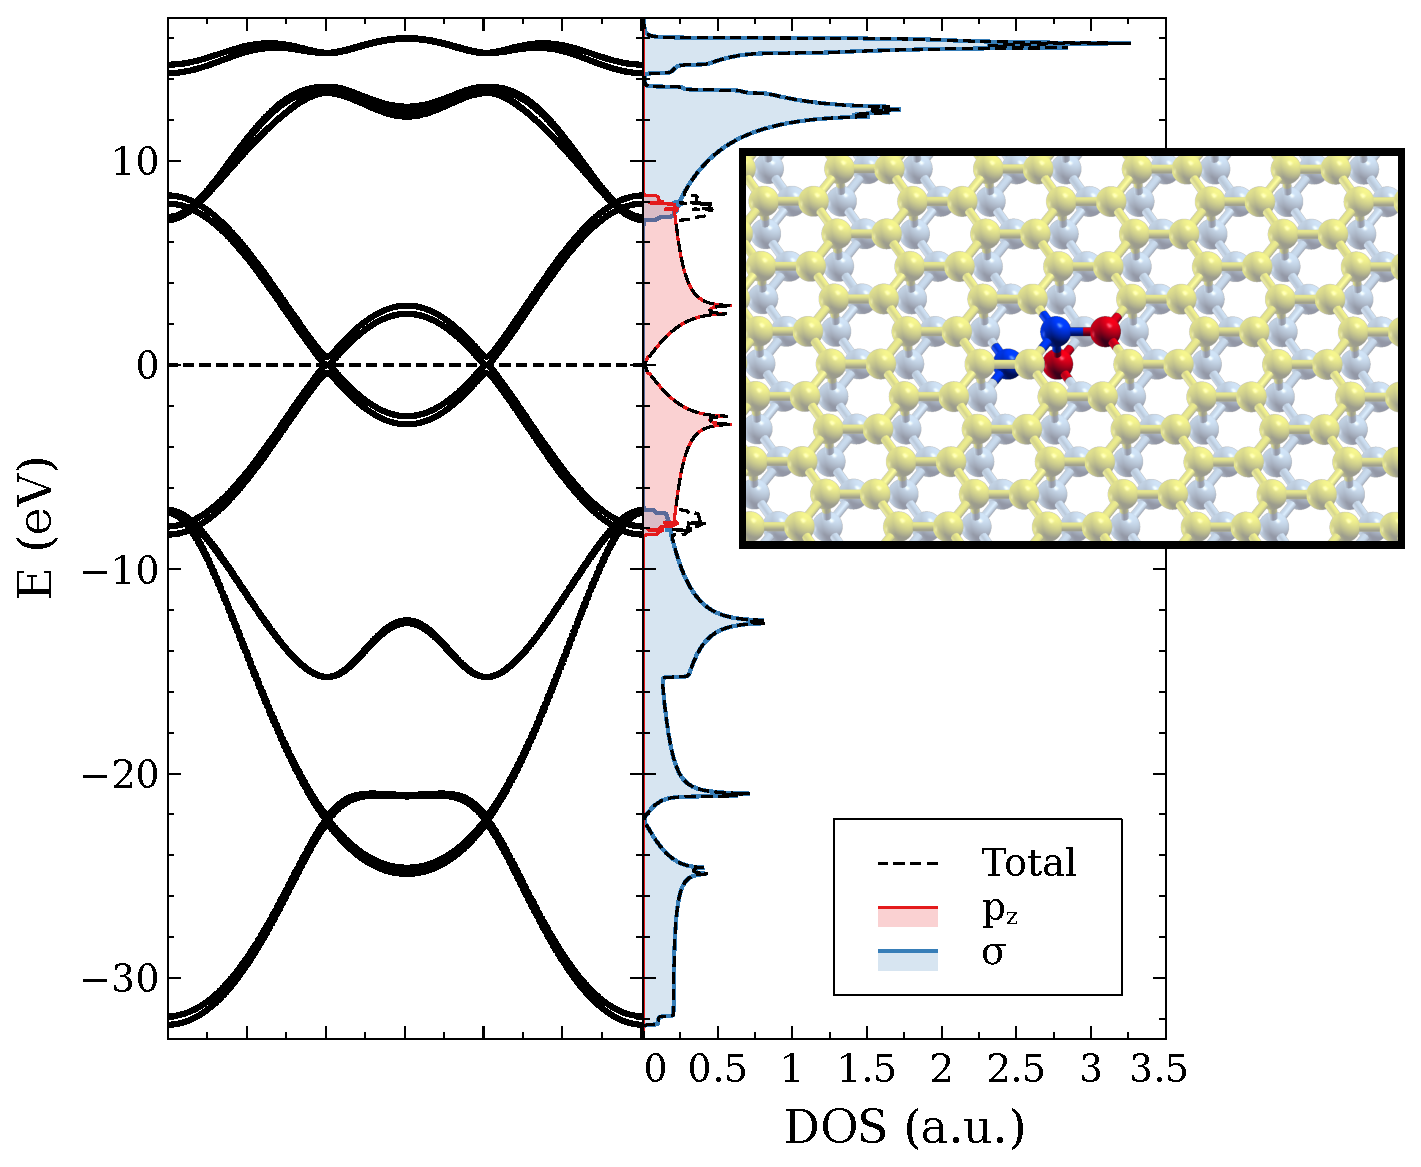
\includegraphics{chapter06/figures/bilayer_bandDOS.pdf}
\vspace{-5pt}
\caption{Band structure and \ac{dos} of graphene bilayer}
\label{bilayer}
\end{figure}
\FloatBarrier
%~~~~~~~~~~~~~~~~~~~~~~~~~~~~~~~~~~~~~~~~~~~~~~~~~~~~~~~~~~~%
The color in the bands in Fig.~\ref{bilayer} show the $p_z$ component of each of the eigenvalues. Notice that in the bilayer the $p_z$ manifold is no longer decoupled from the rest of the orbitals (for instance there is a finite hopping between $p_z$ orbitals from one layer and $s$ orbitals of the other), nevertheless close to the Fermi energy the approximation of considering only $p_z$ orbitals is still justified.
The general aspect of the \ac{dos} is similar to that of the graphene but it is important to notice that at $E=0$ the \ac{dos} is now finite.

\subsection{Effect of the electric field}
When an electric field is applied to graphene bilayer it will affect the Hamiltonian as a diagonal term with $\pm E$ value for each layer. Such a term opens a gap in the \ac{dos} as it is shown in figure~\ref{bi_Efield}

%~~~~~~~~~~~~~~~~~~~~~~~~~~ FIGURE ~~~~~~~~~~~~~~~~~~~~~~~~~%
\begin{figure}[h!]
  \centering
  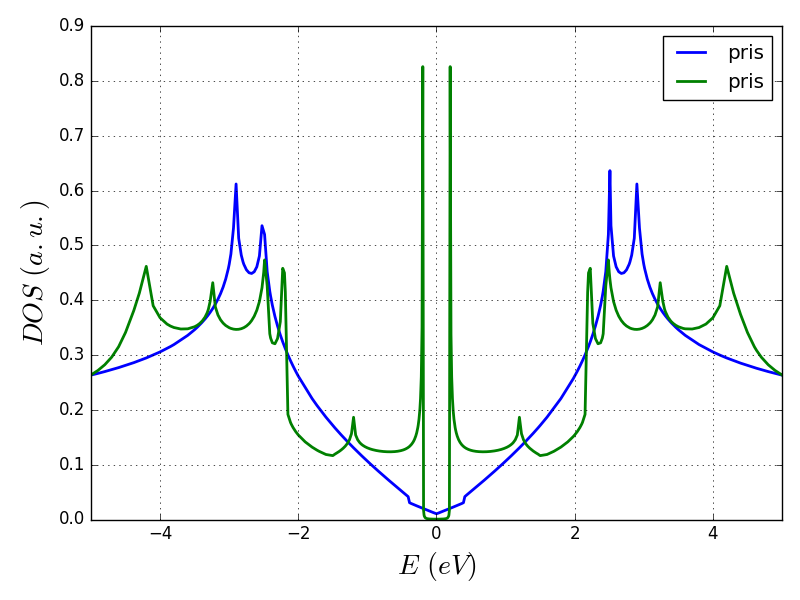
\includegraphics{chapter06/figures/bilayer_dos_E.png}
  \vspace{-5pt}
  \caption{\ac{dos} of a bilayer graphene system in the absence (blue line) and presence (green line) of an electric field $E=0.5$} %XXX UNITS
  \label{bi_Efield}
\end{figure}
\FloatBarrier
%~~~~~~~~~~~~~~~~~~~~~~~~~~~~~~~~~~~~~~~~~~~~~~~~~~~~~~~~~~~%

Analogously to the discussed scenario of a vacancy in (monolayer) graphene, the introduction of a vacancy also results in the appearance of a ``zero energy state''. In the presence of an external electric field the impurity state will not appear at $E=0$ but shifted in energy as shown in fig.~\ref{dos_bi_dfct}

%~~~~~~~~~~~~~~~~~~~~~~~~~~ FIGURE ~~~~~~~~~~~~~~~~~~~~~~~~~%
\begin{figure}[h!]
\centering
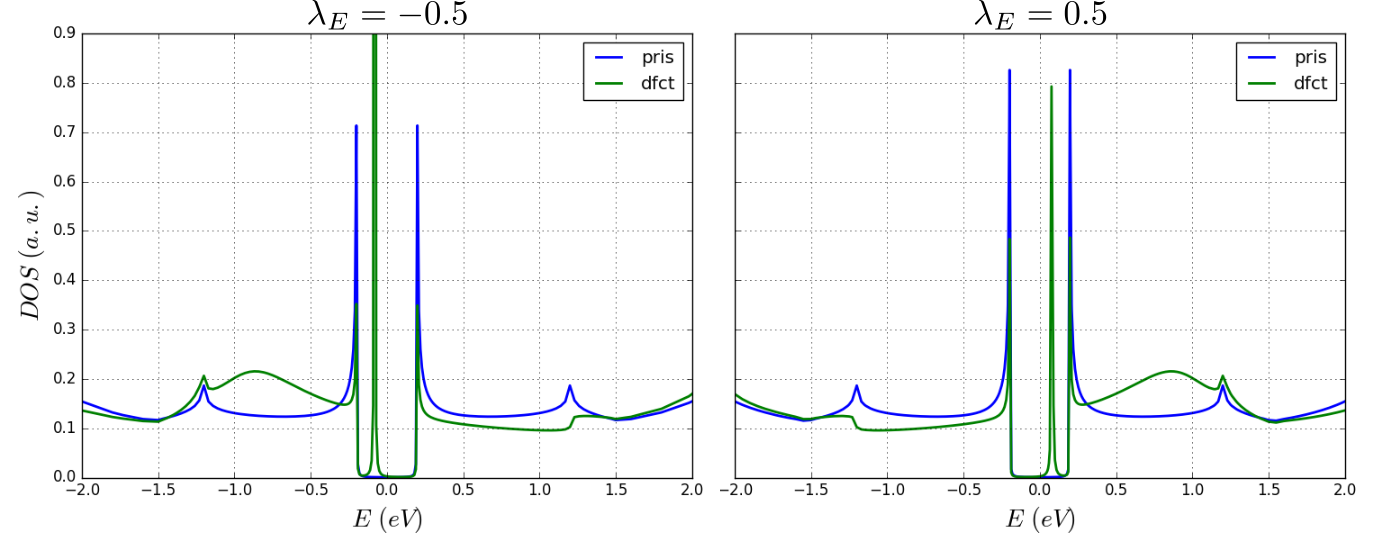
\includegraphics{chapter06/figures/bilayer_dos_dfct.png}
\vspace{-5pt}
\caption{\ac{dos} of bilayer graphene with (green line) and without (blue line) a vacancy in the presence of an external electric field. The left and right panels have been calculated for electric fields of opposite sign, notice that }
\label{dos_bi_dfct}
\end{figure}
\FloatBarrier
%~~~~~~~~~~~~~~~~~~~~~~~~~~~~~~~~~~~~~~~~~~~~~~~~~~~~~~~~~~~%

















The position where the adatom is introduced now is important since one of the sublattices of each layer is fully connected to the other layer. All the possibilities for the H chemisorption are depicted in figure\red{FIG}. We will consider only the structure (b).

%~~~~~~~~~~~~~~~~~~~~~~~~~~ FIGURE ~~~~~~~~~~~~~~~~~~~~~~~~~%
\begin{figure}[h!]
\centering
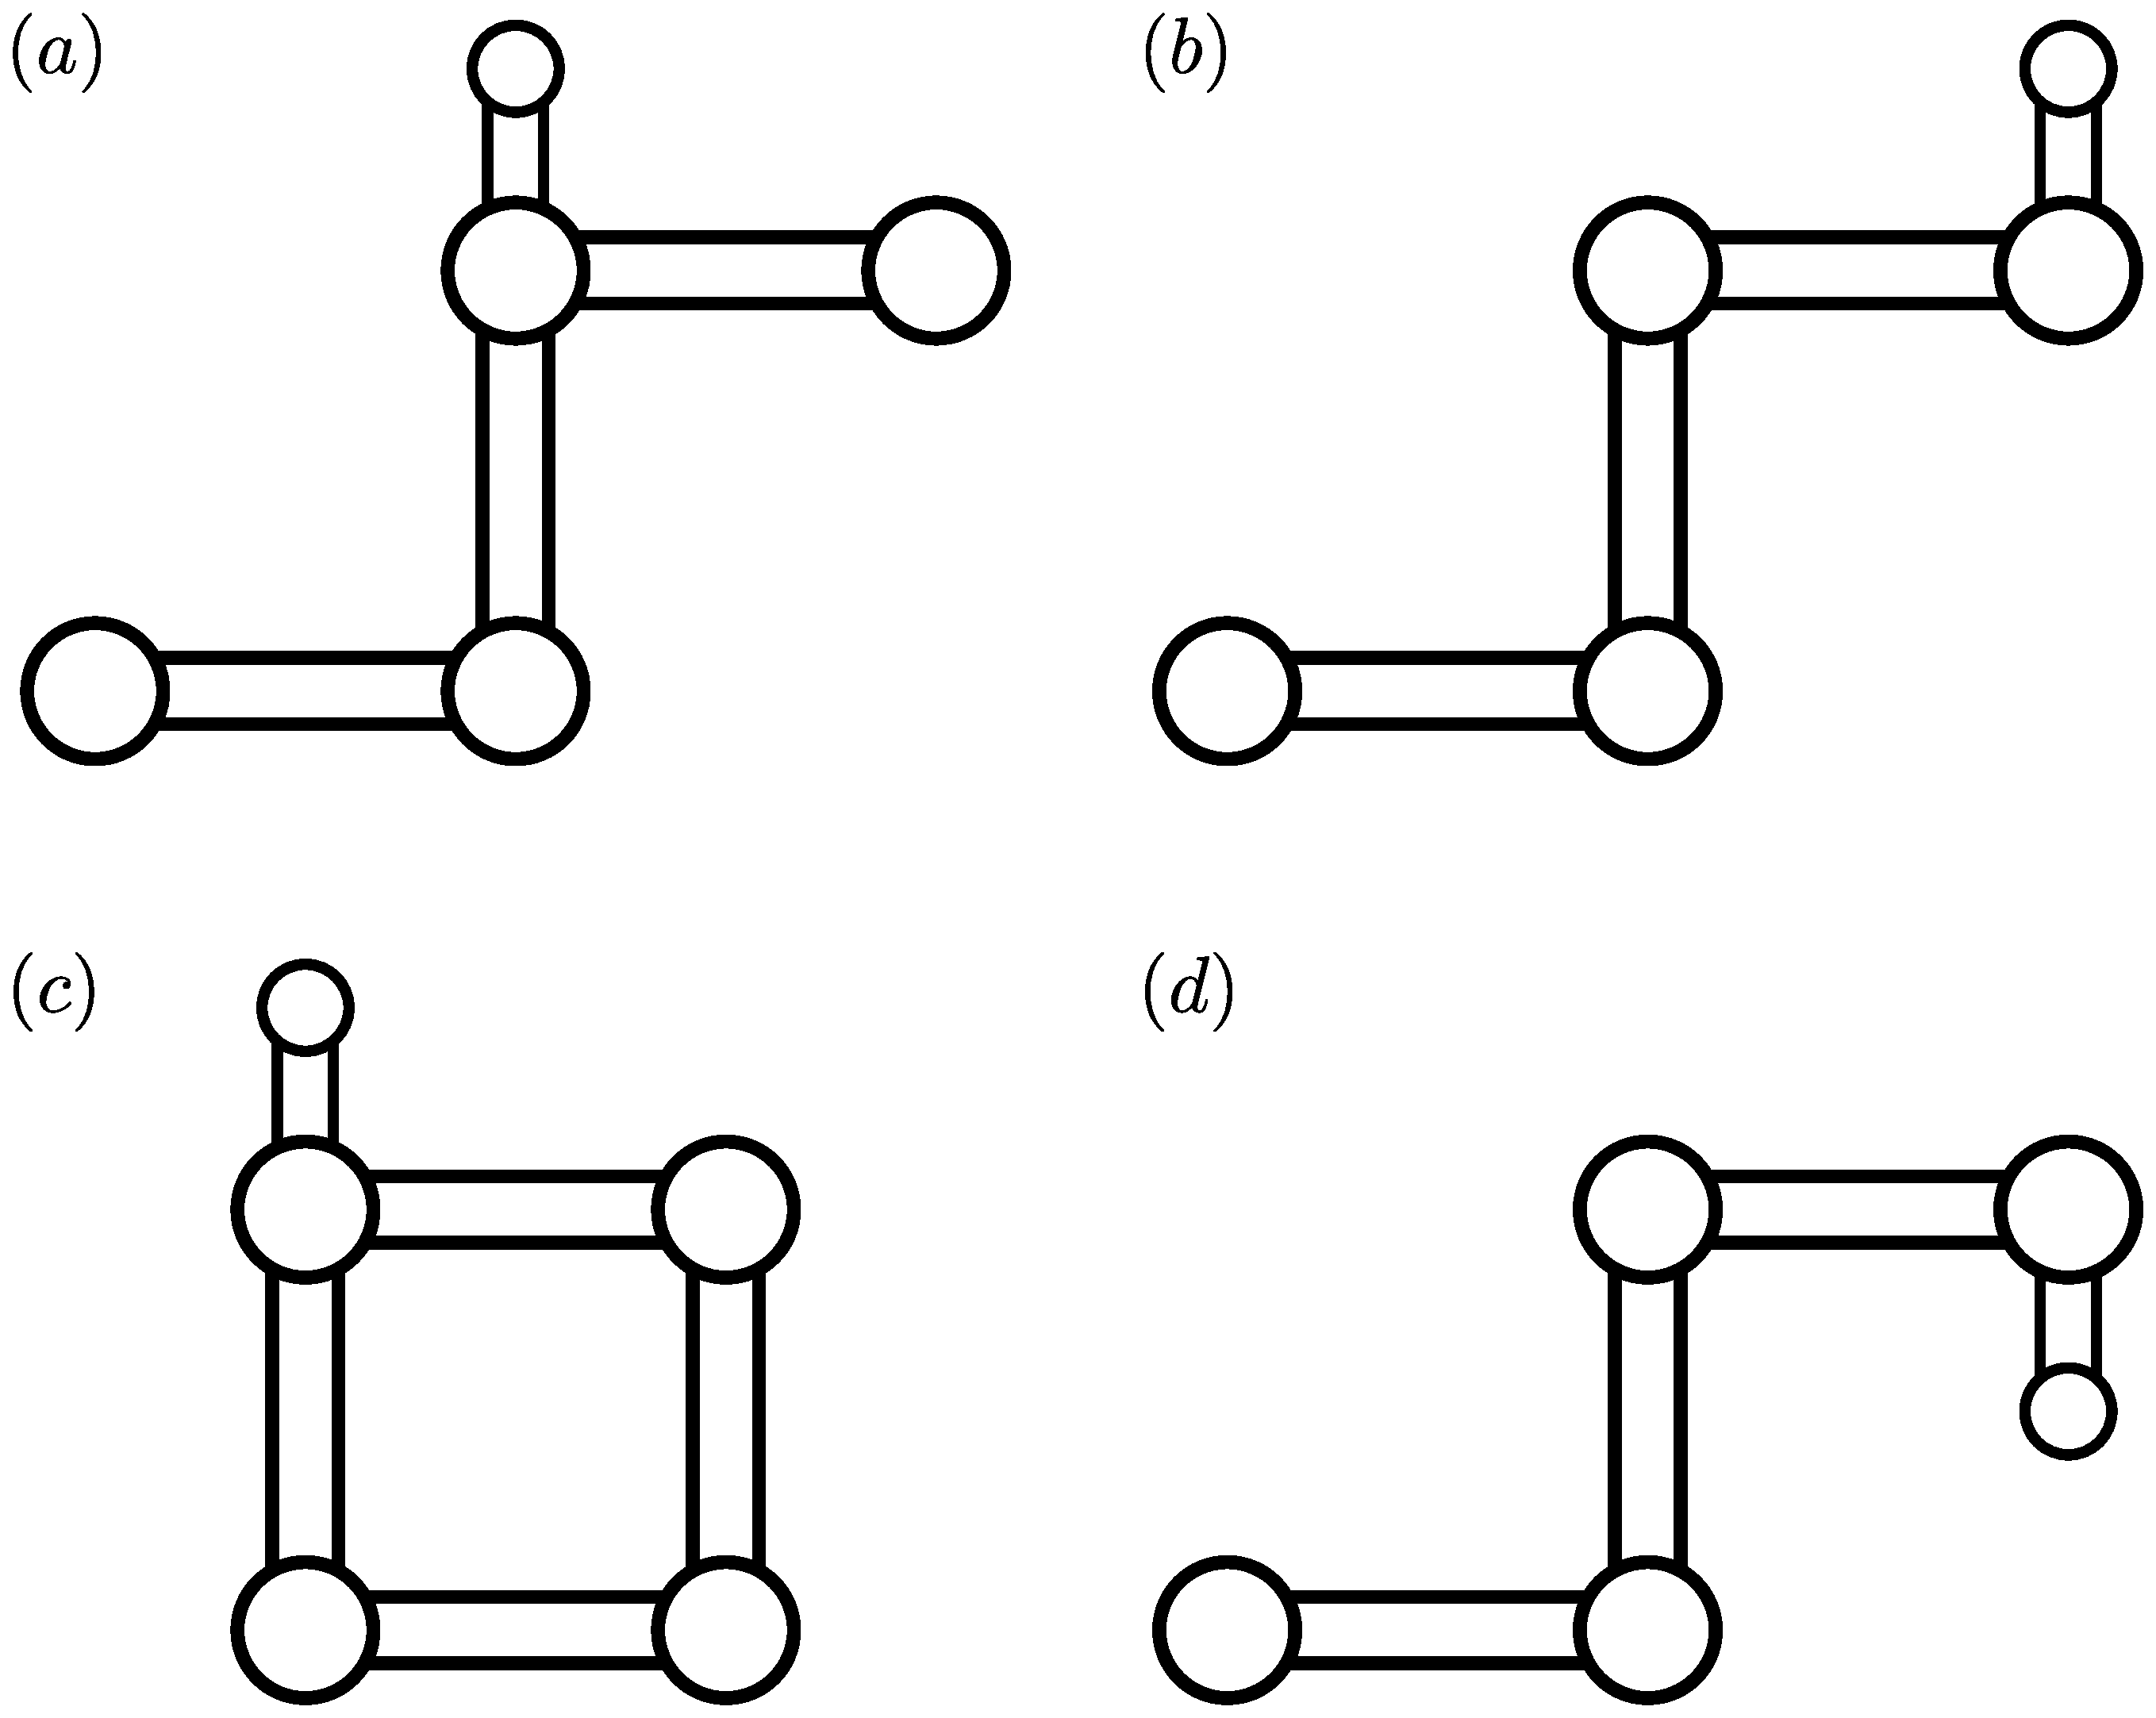
\includegraphics{chapter06/figures/bilayer_H.pdf}
\vspace{-5pt}
\caption{All opssible atomic strucutre for chemisorbed H}
\end{figure}
%~~~~~~~~~~~~~~~~~~~~~~~~~~~~~~~~~~~~~~~~~~~~~~~~~~~~~~~~~~~%



\subsection{Electric control of the hyperfine interaction}
Electric control of the hyperfine with the bias in the bilayer.
%~~~~~~~~~~~~~~~~~~~~~~~~~~ FIGURE ~~~~~~~~~~~~~~~~~~~~~~~~~%
\begin{figure}[h!]
\centering
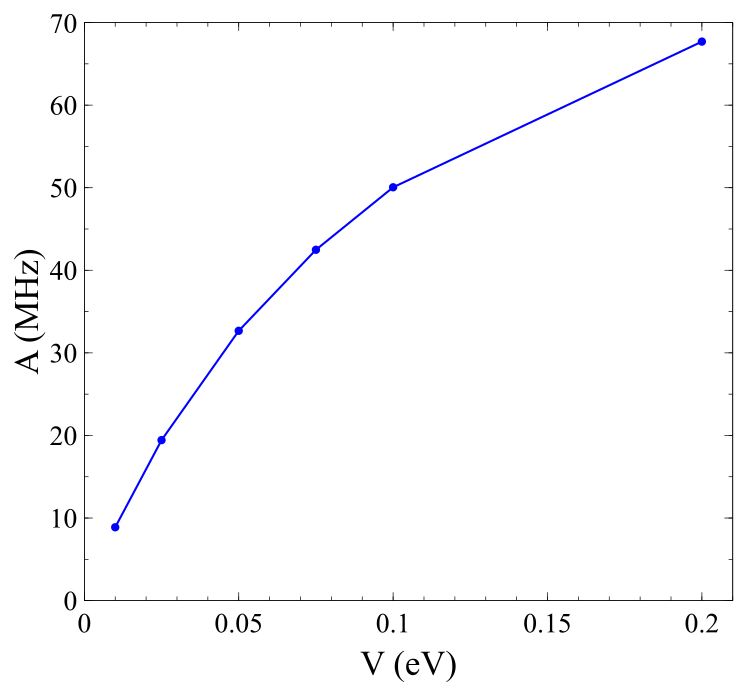
\includegraphics{chapter06/figures/hyperfine.png}
\vspace{-5pt}
\caption{Hyperfine dependence with the bias voltage.}
\end{figure}
\FloatBarrier
%~~~~~~~~~~~~~~~~~~~~~~~~~~~~~~~~~~~~~~~~~~~~~~~~~~~~~~~~~~~%

A similar behavior can be seen from the gap.
%~~~~~~~~~~~~~~~~~~~~~~~~~~ FIGURE ~~~~~~~~~~~~~~~~~~~~~~~~~%
\begin{figure}[h!]
\centering
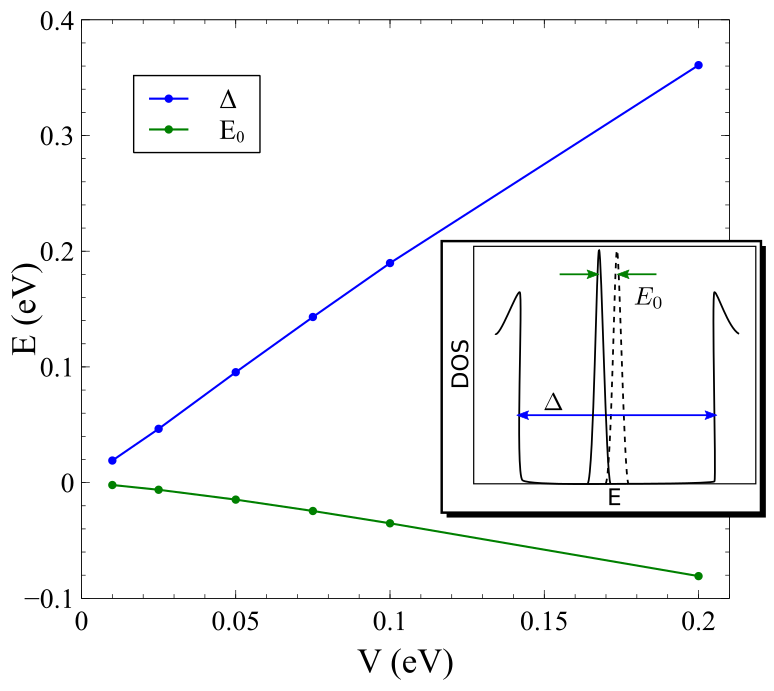
\includegraphics{chapter06/figures/gap.png}
\vspace{-5pt}
\caption{Dependence of the gap and the energy of the resonance with the bias voltage.}
\end{figure}
\FloatBarrier
%~~~~~~~~~~~~~~~~~~~~~~~~~~~~~~~~~~~~~~~~~~~~~~~~~~~~~~~~~~~%



\subsection{Electric control of exchange}
Electric control of the exchange with with the bias between adatoms?
%~~~~~~~~~~~~~~~~~~~~~~~~~~ FIGURE ~~~~~~~~~~~~~~~~~~~~~~~~~%
\begin{figure}[h!]
\centering
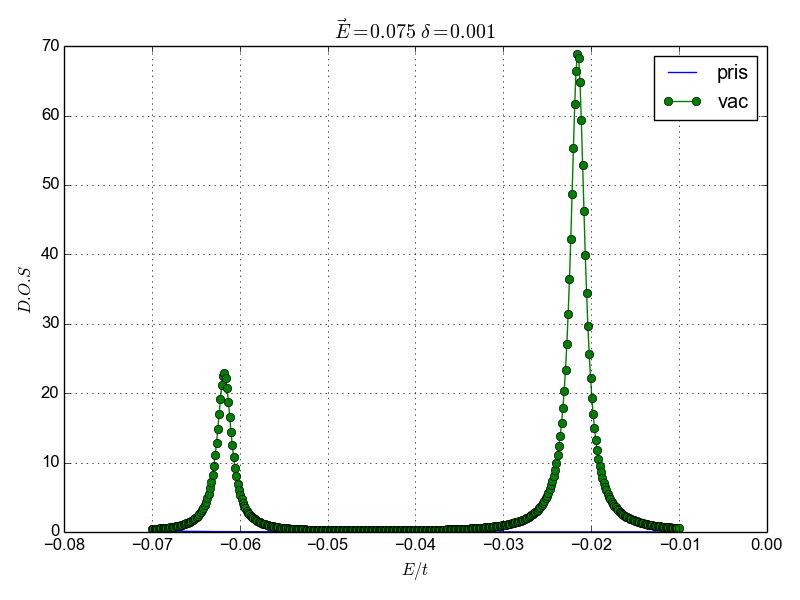
\includegraphics{chapter06/figures/4x4_l0_075.png}
\vspace{-5pt}
\caption{DOS in the gap for a bilayer with $E=0.075$ for a $4\times4$ unit cell}
\end{figure}
\FloatBarrier
%~~~~~~~~~~~~~~~~~~~~~~~~~~~~~~~~~~~~~~~~~~~~~~~~~~~~~~~~~~~%
\begin{equation}
  J = U \sum_i\sum_{k,k'} |\psi_0(i)|^2\psi_k(i)\psi_{k'}(i)
\end{equation}



\section{Spin Lifetime}
We are interested in evaluating the lifetime...

We consider a small sub-system, $\mathcal{A}$, interacting with a reservoir $\mathcal{R}$. The Hamiltonian of the complete system is
\begin{equation}
  H = H_{\mathcal{A}} + H_{\mathcal{R}} + V
\end{equation}
where $H_{\mathcal{A}}$ and $H_{\mathcal{R}}$ are the sub-system and reservoir hamiltonian respectively , and $V$ is the interaction between them.

The density operator, $\rho$, for the complete system ($\mathcal{A} + \mathcal{R}$) satisfies the evolution
\begin{equation}
  \partial_t \rho(t) = \frac{1}{i\hbar}\left[H,\rho(t)\right]
\end{equation}
or, in the interaction representation:
\begin{equation}
  \partial_t \tilde{\rho}(t) =
  \frac{1}{i\hbar}\left[\tilde{V}(t),\tilde{\rho}(t)\right]
\end{equation}
with
\begin{equation}
  \tilde{\rho}(t) = e^{i(H_A+H_R)t/\hbar} \rho(t) e^{-i(H_A+H_R)t/\hbar}
\end{equation}



\section{Read-Out/Other processes}
